\chapter{Review of Methodology}\chaplabel{2}

This chapter aims to conduct a preliminary task analysis and paper review, then a systematic introduction to possible methods for solving the given task is provided. A literature review on common methods will be presented to provide a comprehensive understanding of the topic.

\section{Related Work}

The detection of the roller shutters can surely be realized by human eyes and manual measurement. However, different lighting and weather conditions, for example, during the night or on rainy days, may have a huge impact on the preciseness of human eye recognition. In addition, it may cost a lot of time and labor to realize round-the-clock detection. To improve efficiency and reduce costs, previous studies have suggested the use of computers to replace humans in some aspects of these visual tasks, that is, the introduction of \textbf{machine vision}.

Few previous studies focused exactly on detecting the roller shutters of windows. However, as the principles and detection requirements are similar to many other parts of a building, candidate methods for this bachelor thesis can be referenced from studies that aimed to detect doors, windows, or other basic building components.

Digital signal processing is a common and traditional tool used for solving machine vision tasks. In a previous work, Jin et al. applied a content-based object detection approach to window detection, which utilized gradient transforms to detect edges \cite{jin2001content}. Similarly, Recky et al. used an extended gradient projection method for detecting windows, and introduced a facade color descriptor based on k-means clustering in a CIE-Lab color space \cite{recky2010windows}. Sirmacek et al. utilized a set of steerable filters for L-shape features and perceptual organization rules to detect windows and doors on a rectified thermal image of the building \cite{sirmacek2011detection}. These studies all showed promising experimental results, but the error rates were mainly attributed to different lighting conditions and window reflections. Therefore, characterizing the various appearances of real-world surfaces remains a challenging task for these legacy approaches. 

As artificial intelligence advances, machine learning and deep learning algorithms have been applied to various machine vision tasks. Wang et al. designed a robust classifier for window detection in facades using the traditional machine learning algorithm Gentle AdaBoost. In recent studies, You Only Look Once (YOLO) has been used to train prediction models for tasks such as door detection in convenience stores. Researchers in a 2021 study utilized YOLOv4, which is considered state-of-the-art, and optimized the model to distinguish between convenience store glass doors and glass walls by incorporating surrounding objects in the scene. Biyomi et al. also used YOLOv5 for building envelope detection and compared its performance to other methods in a recent study. These studies suggest that applying machine learning and deep learning algorithms can lead to higher detection accuracy and can handle various scenarios. However, the training process may require large amounts of data and equipment, and may take longer than traditional digital signal processing methods.

As seen from the timeline of related studies, applying deep learning methods to machine vision tasks has become the main trend. However, digital signal processing and traditional machine learning methods can be more efficient in certain detection problems. Additionally, previous studies have primarily focused on determining the location of the target object, with the parameters of the target object itself being less crucial. In contrast, this bachelor thesis considers not only "where" but also "how much" as equally crucial. Since it is still unclear which method would be most appropriate for the current task, the following sections will introduce these methods accordingly.

\section{Machine Vision}

Machine vision is a subcategory of computer vision, which is proposed by David Marr in his book vision\cite{marr_vision_2010}. It refers to the technology and methods used to provide imaging-based automatic inspection and analysis for such applications as automatic inspection, process control, and robot guidance, usually in industry \cite{steger_machine_2018}.

The primary purpose of machine vision is to create models and data extracts and information from images \cite{wiley_computer_2018}. Machine vision works by using an algorithm and optical sensors to stimulate human visualization to automatically extract valuable information from an object. Image processing and pattern recognition become two indispensable components for machines to output image understanding. Many techniques from artificial intelligence also play important roles in all aspects of computer vision \cite{jain_machine_1995}.

As shown Figure \ref{fig:1}, based on the review of previous studies, a machine vision task can generally be solved by using the traditional \textbf{Digital Signal Processing (DSP)} method, or \textbf{Machine Learning} related methods.

\begin{figure}[h]
  \centering
  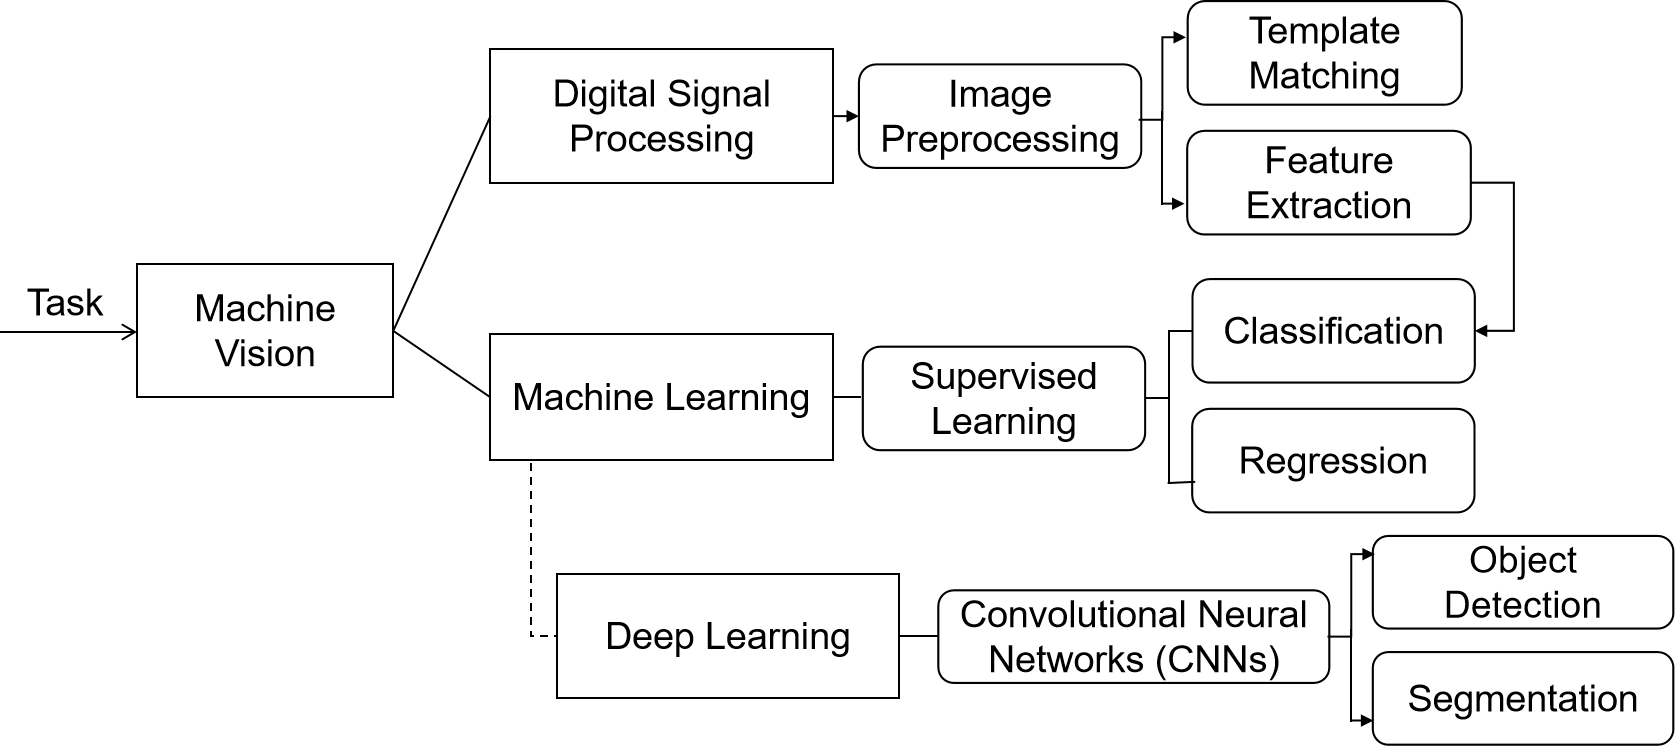
\includegraphics[width=1\textwidth]{Figures/Methodology Overview.png}
  \caption{Methodology Overview}
  \label{fig:1}
\end{figure}

\section{Digital Signal Processing}

Digital Signal processing techniques can be applied to process digital images. A digital image is a two-dimensional matrix of pixel points, each with certain brightness and color information. By using DSP techniques, we can analyze these pixel points to extract useful information. Such process is called digital image processing. It mainly includes the following aspects: Image preprocessing, feature extraction and template matching.

\subsection{Image Preprocessing}

Due to the complexity of the acquisition environment and lighting, the quality of the image can be greatly disturbed, which in turn affects the accuracy of recognition. Therefore, before the image is recognized, the necessary preprocessing operations need to be performed. Basic preprocessing operations include graying, binarization, smoothing, enhancing, scaling, rotating and edge detection.

\textbf{Graying} is the process of changing the image to grayscale, while \textbf{binarization} changes the grayscale image into a grayscale image with values of 0 and 255. These two operations reduce the amount of data in the image and simplifies the image processing. \textbf{Smoothing} removes detailed information from images to reduce noise and image distortion, where median filter is a commonly used technique. \textbf{Enhancing} aims to improve the contrast, brightness, and detail of images, making them sharper and easier to see. Histogram Equalization is the state-of-art. \textbf{Scaling} and \textbf{rotating}, as their names indicate, change the size, direction, angle of the image for better follow-up processing and analysis. 

\textbf{Edges} are very important features of an image in machine vision. This is because edges represent the demarcation line between different regions, and such division is crucial for segmentation and object recognition. \textbf{Edge detection} is the operation to detect such edges in the preprocessing stage. Canny algorithm \cite{canny_computational_1986} is a widely used gradient-based edge detection algorithm which can accurately detect edges in the image with good noise immunity and efficient performance. Figure \ref{fig:2} shows the effect of aforementioned preprocessing operations. 

\begin{figure}[h]
  \centering
  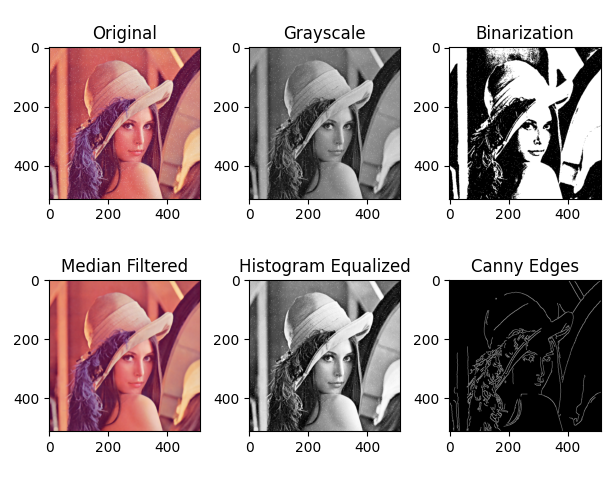
\includegraphics[width=0.7\textwidth]{Figures/Image Preprocessing.png}
  \caption{Effect of multiple preprocessing operations}
  \label{fig:2}
\end{figure}

\subsection{Template Matching}

\textbf{Template matching} refers to finding the part of the test image that is similar to the template image by comparing between the template image and the test image, which is achieved by calculating the similarity between the template image and the target in the test image, and can quickly locate the predefined target in the test image. A template can be an example, an instance; esp. a typical model or a representative instance  \cite{brunelli2009template}.

Template matching is very similar to the principle of convolution, the template slides on the original image from the origin, calculates the degree of difference between the template and the place where the image is covered by the template, then the result of each calculation is put into a matrix and output as the result. After that maximum value in the similarity matrix is found, and this will give a position at which the input image matches the template image to the highest degree. That position is then be used to position the area which matches the template. Figure \ref{fig:3} shows an example of template matching.

Template matching is a simple and efficient way to detect the target object. Compared to 
machine learning techniques, template matching does not require a large amount of training data and can therefore be used when the amount of data is limited. However, such method is sensitive to image transformations, and even slight environment changes would cause the failure, letting alone tackling the problem of occlusion. In order to improve the stability and accuracy of the algorithm, techniques like scale and rotation invariant feature detection are used to extract features from the image.

\begin{figure}[h]
  \centering
  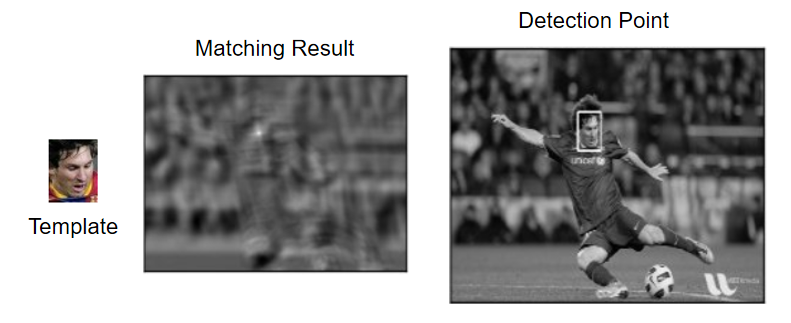
\includegraphics[width=1\textwidth]{Figures/Template_Matching.png}
  \caption{An example of template matching in OpenCV} \cite{opencv}
  \label{fig:3}
  
\end{figure}


\subsection{Feature Extraction}

Feature extraction is the basis of object recognition, which can extract important information from images like feature points. These feature points can be kept constant at different scales and angles, thus improving the accuracy of object recognition and classification. Several common feature extraction techniques are described below:

\textbf{Harris corner detector} \cite{harris1988combined}, as the name infers, is used to extract corner feature points by calculating the difference in gray value between a pixel point in the image and its surrounding pixel points. 

\textbf{scale-invariant feature transform (SIFT)} \cite{lowe1999object} transforms an image into a large collection of feature vectors, each of which is invariant to image translation, scaling, and rotation, partially invariant to illumination changes, and robust to local geometric distortion. Several improvements have been made in its improved algorithm \textbf{Speeded-up robust features (SURF)} \cite{bay2008speeded}.

\textbf{Oriented FAST and rotated BRIEF (ORB)} \cite{rublee2011orb} is a faster, more robust local feature detector modified from SIFT and SURF to detect features points in images and generate descriptors. However, it is less robust to different lighting conditions and occlusion.

After feature descriptors are extracted, they are used as input to train the classifier which is then used for classification or object detection. Related machine learning terms will be explained in the next section.

\section{Machine Learning}

\textbf{Machine learning} is a sub-field of artificial intelligence that is concerned with building useful algorithms rely on a collection of examples, no matter naturally or artificially generated \cite{burkov2019hundred}.

\subsection{Supervised Learning}

\textbf{Supervised learning} is one of the categories and the most common learning method of machine learning. The aim of supervised learning is to build a model that makes predictions based on evidence in the presence of uncertainty. A supervised learning algorithm takes a pre-labelled input data and known responses to the data (output) and trains a model to generate reasonable predictions for the response to new data. Such a predictive model can be based on two techniques: classification and regression, predicting discrete and continuous responses respectively. Most image-focused pattern-recognition tasks usually depend on classification using supervised learning.

\subsection{Classification}

\textbf{Classification} is the task which automatically assigning a discrete label to an unlabeled example, for example, assigning a given email to the "spam" or "non-spam" class. \cite{burkov2019hundred}

A classification problem in machine learning is typically addressed through the use of a classification learning algorithm. These algorithms take a set of labeled examples as input and generate a model that can be used to predict the label of a new, unlabeled example. The output of the model can be either a directly assigned label, or a numerical value that can be interpreted by an analyst to deduce the label.

\textbf{Support Vector Machine (SVM)} is a type of classifier commonly used to tackle two-group classification problems. The machine conceptually implements the following idea: input vectors are non-linearly mapped to a very high-dimension feature space \cite{cortes1995support}. In machine learning, the boundary separating the examples of different classes is called the decision boundary \cite{burkov2019hundred}. The algorithm aims to construct a maximally spaced hyperplane during the training so that the decision boundary has the maximum margin between the closest samples. 

The evaluation of the classification result can be done by a \textbf{confusion matrix}, which can classify the test data into four categories: true positives (TP) , false positives (FP), true negatives (TN) and false negatives (FN). Correct Classification Rate (CCR) , a common assessment metric of classification models, can then be calculated as follow:

$$
   \text{CCR} = \frac{\text{TN} + \text{TP}}{\text{FN} + \text{FP} + \text{TP} + \text{TN}}
$$

An example is shown in figure \ref{fig:4}. As can be seen, the decision boundary L1 is set too close to the training samples, while L2 obtained by SVM algorithm maintains the largest margin. Two boundaries may make different predictions to the test sample marked in the figure, and these results are evaluated differently in the confusion matrix (FN for L1 and TP for L2). This can show how L2 may obtain a better CCR as similar test samples increases.

\begin{figure}[h]
  \centering
  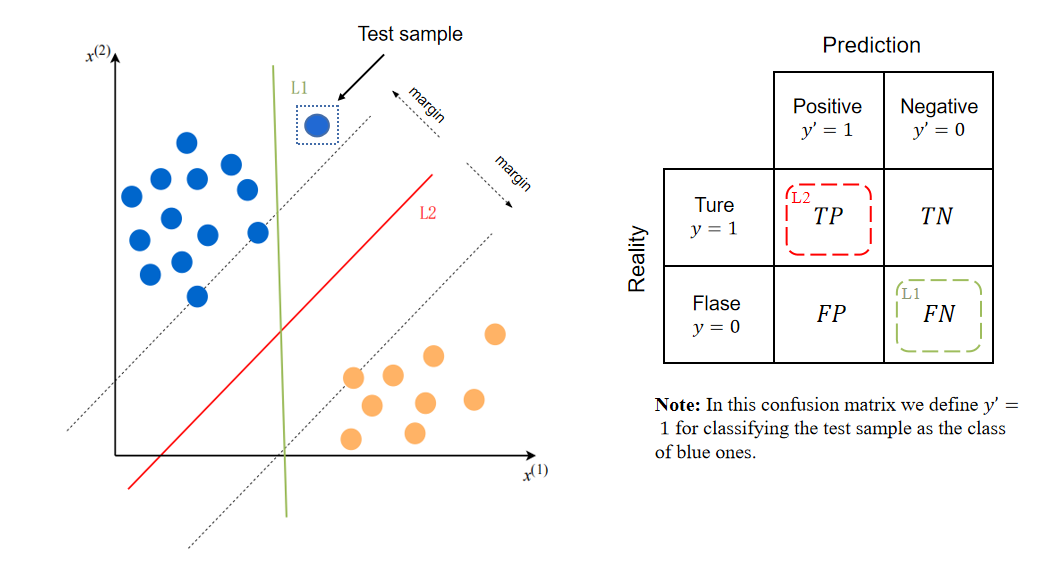
\includegraphics[width=0.8\textwidth]{Figures/SVM and confusion matrix.png}
  \caption{An example of SVM decision boundary (left) and the confusion matrix (right). L1 fails to classify the marked test sample correctly}
\cite{burkov2019hundred}
  \label{fig:4}
\end{figure}

\subsection{Regression}

\textbf{Regression} is the task of predicting a real-valued label (often called a target) given an unlabeled example, for example, estimating stock price \cite{burkov2019hundred}.

In supervised learning, a regression problem chooses a regression algorithm to take a collection of labeled examples as inputs and produces a model that can take an unlabeled example as input and output a target. The relation between predicted output and input can be expressed as $ y' = f (x) $. Based on the function, a regression problem can be classified as linear regression, polynomial regression, etc. During the training of a regression model, \textbf{loss function} is used to evaluate the performance by calculating the error between predicted and true values. Mean Squared Error (MSE) is a common loss function, which can be calculated by $ MSE = \frac{1}{n}\sum_{i=1}^{n}(y_i - \hat{y}_i)^2$. The smaller the MSE, the better the performance of the model will be. Figure \ref{fig:5} depicts an example of a linear regression model and the corresponding MSE.

\begin{figure}[h]
  \centering
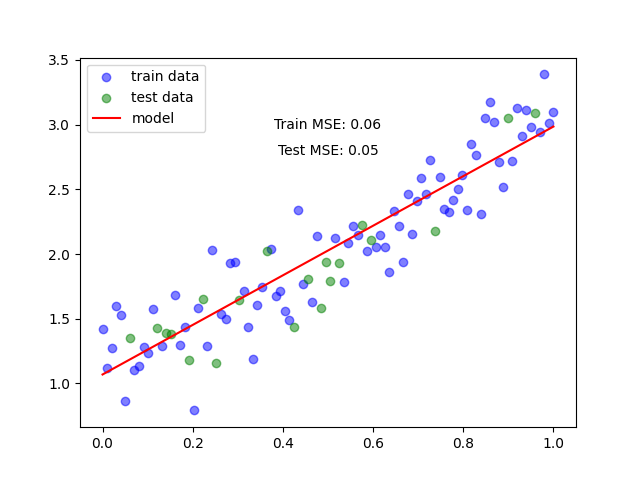
\includegraphics[width=0.5\textwidth]{Figures/Linear Regression.png}
  \caption{An example of a linear regression model}
  \label{fig:5}
\end{figure}

In order to minimize the loss function of the model, \textbf{gradient descent algorithm} is used to obtain the best model parameters. Gradient descent algorithm is an iterative optimization algorithm that reduces the value of the loss function by calculating the partial derivatives (gradient) of the loss function with respect to the model parameters and updating the model parameters along the negative gradient direction. The algorithm is used to continuously update the model parameters, and the optimal regression model can be gradually fitted to minimize the error between the prediction result and the true value.

Traditional machine learning classification and regression methods can largely improve the adaptability to different scenarios and tasks compared to the traditional digital signal processing. However, their generalization capabilities are still insufficient, while a large number of manual rules still need to be designed for feature extraction and dealing with occlusion.


\section{Artificial Neural Networks (ANNs) and Deep Learning}

\textbf{Artificial neural networks (ANNs)} is a very useful tool in supervised learning and is the foundation of deep learning. ANNs are computational processing systems of which are heavily inspired by way biological nervous systems (such as the human brain) operate. ANNs are mainly comprised of a high number of interconnected computational nodes, which we name as neurons. These neurons work distributively to collectively learn from the input in order to optimise its final output.

Figure \ref{fig:6} shows the architecture of a simple ANN and how a neuron processes its input. For every neuron, it calculates the sum of every input, which is the output of each neuron in the previous layer, with \textbf{weights} set to each input to measure its influence on the result. A \textbf{bias} is also set to adjust the intermediate result for \textbf{activation} afterward. The goal of activation is to add non-linear features into the output of a neuron, which helps neural networks discover and learn complex patterns, and to normalize such output to be an input of the next layer. Rectified Linear Unit (ReLU) is one of the commonly used activation functions, which simply turns all negative output values to 0.

An ANN is generally composed of three types of layers. The input layer loads inputs in the form of a multidimensional vector to the input layer, and distribute them to the hidden layer. The hidden layer will then make decisions from the previous layer and weigh up how a stochastic change within itself detriments or improves the final output, and this is referred to as the process of learning. Having multiple hidden layers stacked upon each-other is commonly called deep learning \cite{oshea_introduction_2015}.

\begin{figure}[h]
  \centering
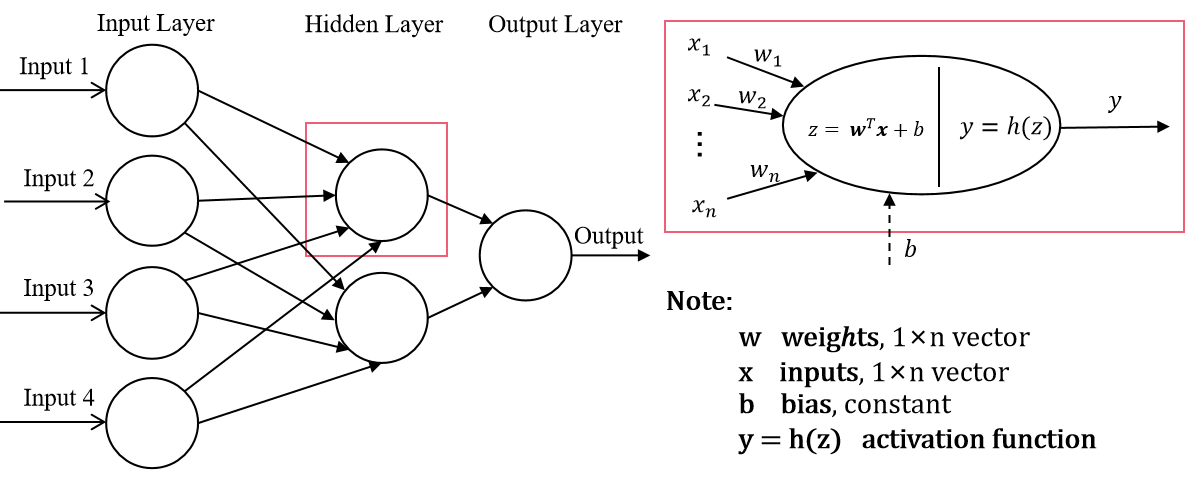
\includegraphics[width=1\textwidth]{Figures/ANN-architecture.png}
  \caption{The architecture of a simple ANN network}
  \label{fig:6}
\end{figure}

One of the largest limitations of traditional forms of ANNs is that when computing image data, they tend to struggle with the computational complexity. This is because each neuron in fully-connected layers needs to be connected to all neurons in the previous layer, and this require a lot of computation to deal with the huge number of weights each neuron provides for every single pixel. Besides, even if the computing power is unlimited, the complexity will cause another problem: overfitting, which occurs when a model is trained too well on a particular data set, to the extent that it starts to fit the noise or random fluctuations in the data rather than the underlying patterns or trends, resulting in poor performance on new, unseen data. In order to reduce the complexity of ANNs, \textbf{Convolutional Neural Networks (CNNs)} is introduced. 

\subsection{Convolutional Neural Networks (CNNs)}

CNNs are analogous to traditional ANNs in that they are comprised of neurons that self-optimise through learning. The notable differences between two networks are their architectures, which makes CNNs more capable in the field of pattern recognition within images.

Figure \ref{fig:6} depicts the architecture of a general CNN. The basic functionality of this example CNN can be broken down into three key areas: convolutional layers, pooling layers and fully-connected layers.

\begin{figure}[h]
  \centering
  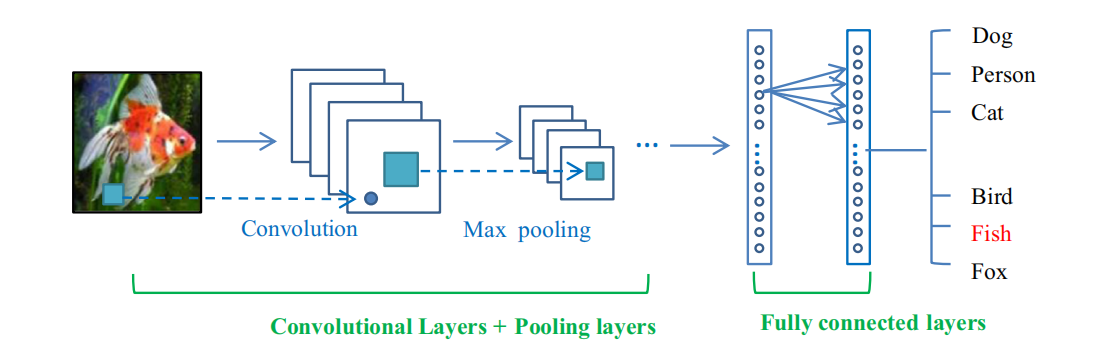
\includegraphics[width=1\textwidth]{Figures/CNN-architecture.png}
  \caption{The pipeline of the general CNN architecture \cite{guo_deep_2016}}
  \label{fig:6}
\end{figure}

As can be implied from the name, \textbf{convolutional layers} play a vital role in how CNNs operate. Its main task is to extract features from the original input image by convolution operations. The output of the convolution layer can be used as the input of the next layer. 

Feature extraction in the convolutional layers is realized by several learnable convolution \textbf{kernels}, which are used to convolve the input image to produce an output feature map. In a CNN, each neuron of the convolutional layer uses a kernel to process the input pixels adjacent to it. Every kernel can serve as a filter to extract one specific feature of the input image like edges, corners, etc. Since such filters can be applied to any part of the input image and each type of filters is sharing the same parameters, the number of parameters we required is dramatically decreased. This important feature is called \textbf{parameter sharing}, which can reduce the risk of overfitting and improving the generalization ability of the model. 

During the convolution operation, a kernel is used to slide over the input image, performing one convolution operation at a time, to produce the output feature map. As the input is glided through, the scalar product is calculated for each value in that kernel. Then activation function will be applied, and every kernel will obtain a corresponding activation map, of which will be stacked along the depth dimension to form the full output volume from the convolutional layer.

There are three hyperparameters that control the size of the output volume of the convolutional layer: depth, stride and zero-padding. \textbf{Depth} refers to the number of convolutional kernels in the convolutional layer. \textbf{Stride} is the distance that the filter moves along the input each time. \textbf{Zero-padding} is the simple process of padding the border of the input by setting it zero.

A \textbf{pooling layer} is usually attached after convolutional layers. It contains pooling operations used to reduce the size of the convolutional layer outputs, thereby reducing the model complexity and computing power required. Pooling operations can also improve the robustness and generalization of the model to reduce the risk of overfitting. The most commonly used pooling function is max pooling and average pooling, which take the maximum value in the pooling window as output.

Following several convolutional and pooling layers, \textbf{fully-connected layers} perform the high-level reasoning in CNNs. As the name implies, every neuron in fully connected layer has full connections to all activation in the previous layer. Their activation can then be calculated with a matrix multiplication with a bias offset. The fully connected layer eventually converts the 2D feature map into a 1D vector. The vectors derived can either be fed into a certain number of classifications or can be considered as feature vectors for further processing \cite{voulodimos_deep_2018}. 

The input data is processed through convolutional layers, pooling layers, etc., and finally the prediction result of the model is obtained in the output layer. Such process is defined as forward propagation. However, the predicted value may have deviation from the real one to some extent. In order to diminish such deviation, we need use loss functions to calculate the deviation and updates each parameter by \textbf{back propagation} to minimize the loss. Similar to the process introduced in the regression model training, gradient descent algorithm is also used in back propagation for calculating new weights in that procedure.

\subsection{Object detection}

Object detection aims to automatically identify and localize a specific class of objects from an image or video. The target objects are marked given their locations via \textbf{bounding boxes}. In recent years, the development of deep learning has made significant progress in object detection. Deep learning-based object detection methods include two main types: single-stage detection and two-stage detection.

\textbf{Single-stage detection} requires only one neural network model, performing forward propagation only once to complete the object detection. Therefore, it is an efficient method but with sometimes lower precision. \textbf{You Only Look Once (YOLO)} is a representative single-stage detection algorithm. Its main idea is to divide the feature map obtained from the output of CNN into multiple grids, with each grid predicting a fixed number of bounding boxes and their corresponding object class probabilities. Then, category probabilities and position information of each bounding box are adjusted to obtain the final prediction box. Finally, the Non-Maximum Suppression (NMS) algorithm is applied to remove redundant bounding boxes and obtain the detection results \cite{redmon2016you}. Besides the YOLO series, Single Shot MultiBox Detector (SSD), RetinaNet are another single-stage detection algorithms.

\textbf{Two-stage detection} can offer better accuracy. It involves two steps: proposal generation and detection. In the first stage, a region proposal network generates potential bounding boxes, and in the second stage, features of the proposed regions are extracted and used to classify and refine the boxes. \textbf{Faster R-CNN} and \textbf{Mask R-CNN} are two of the most popular two-stage detection algorithms.

\subsection{Segmentation}

Unlike object detection, segmentation requires classification of each pixel in the image, rather than localizing and classifying only the boundaries of the object. Based on different 
segmentation results, it can be categorized into three types: semantic segmentation, instance segmentation and panoptic segmentation.

\textbf{Semantic segmentation} is an approach detecting, for every pixel, belonging class of the object \cite{guo2019degraded}. For example, all cars in an image are segmented as one object and background as another object. There will be distinctions between two different cars in reality. \textbf{U-Net}, named by its U-shape architecture \cite{ronneberger2015u}, is one of the stage-of-art based on CNN to process semantic segmentation.

\textbf{Instance segmentation} aims to identify the every pixel's belonging of object. It detects each distinct object of interest in the figure. For instance, every car in a figure is segmented as an individual object. \textbf{Mask R-CNN}, which is mentioned above as an object detection algorithm, can also be used in instance segmentation task. 

\textbf{Panoptic segmentation} combines the feature of semantic and instance segmentation. It can identify the belonging class of each pixels, meanwhile distinguishing them based on different instance. However, to realize both features requires processing a large number of object instances and backgrounds simultaneously, and thus requires more resources. \textbf{Panoptic FPN} and \textbf{BlendMask} can be some of the commonly used algorithms.

In Figure \ref{fig:7}, we can see an example of how object detection, semantic segmentation, and instance segmentation can be applied to the same image. The selection of the appropriate method depends on the specific task requirements and scenarios, which will be thoroughly discussed in the following chapter.
\begin{figure}[h]
  \centering
  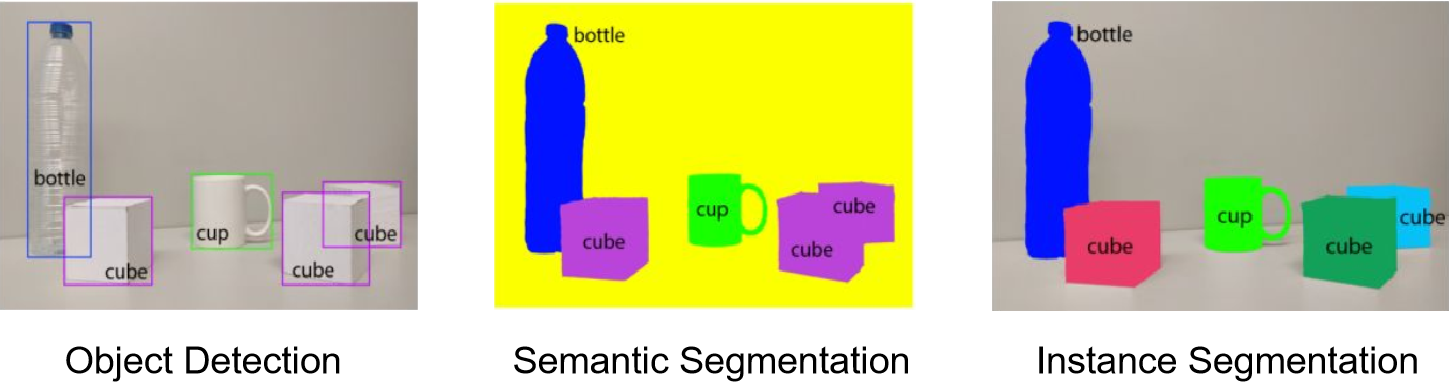
\includegraphics[width=1\textwidth]{Figures/Object detection and segmentation.png}
  \caption{An example of object detection and segmentation}
  \cite{nitish_2017}
  \label{fig:7}
\end{figure} 